The system developed during the project has less than desired performance, and has room for improvement. The poor overshoot performance and the oscillations of the system could be caused by multiple different sources of error. It could be due to an error in our transfer function for the drone, or due to non-linearity in the thrust of the drone versus the height of the drone, or errors in the code comprising the regulator.\\
Due to these sources of error we decided to perform a new step-response test, and got the results as seen in the test report in appendix \ref{ap:drone_secondary_test}.
As described, the main difference of this step-response test, was that the step was performed above 400 mm of height. This was because significant increase in thrust was observed when close to the ground, and increasing the altitude of the step response would eliminate this effect.
During this test we discovered that the drone would in fact hover at 35\% throttle, the value we had used for the initial step-response test.
This prompted us to reconsider the model of the drone, leading us to believe we'd made a mistake in the transfer function for the drone. This was because the step response we were observing in this new test was a constant acceleration, where the previous step we saw would settle on a constant velocity.
Considering this, we tried to model a new transfer function, based on the freebody equation (eq. \ref{eq:new_tf_newton}) for our system

\begin{equation} \label{eq:new_tf_newton}
    M_{drone} * \ddot{z} = F_{thrust} - M_{drone} * g
\end{equation}

Linearizing this transfer function yields equation \ref{eq:new_lin_tf}

\begin{equation} \label{eq:new_lin_tf}
    \hat{F_{thrust}} = M_{drone} * \ddot{z}
\end{equation}

Laplace transforming this gives us our new equation (eq. \ref{eq:new_zf_laplace}) for the height z.

\begin{equation} \label{eq:new_zf_laplace}
    Z(s) = \hat{F_{thrust}}(s) * \frac{1}{M_{drone} * s^2}
\end{equation}

Yielding us the new transfer function \ref{eq:new_tf} from Thrust to vertical velocity.

\begin{equation} \label{eq:new_tf}
    G(s) = \frac{Z(s)}{\hat{F_{thrust}}(s)} = \frac{1}{M_{drone}} * \frac{1}{s}
\end{equation}

where
\begin{itemize}
    \item $Z(s)$ is the vertical position
    \item $\hat{F_{thrust}}$ is the vertical thrust generated by the drone
    \item $M_{drone}$ is the mass of the drone
\end{itemize}

We believe the cause of the additional lift when the drone is close to the ground, is that the drone creates a cushion of air underneath itself. This cushion causes the drone to generate significantly more thrust when close to the ground, causing lower throttle percentages than is required to hover the drone, to accelerate the drone. This was backed up by further tests, showing a 0\% to 35\% throttle step of 1 second would cause the drone to hit the roof of the motion-tracking lab, however manually saving the thrust when an operator hovered the drone, showed that slowly bringing the drone up to a hover, would have the drone hovering at 35\% 

because of the above difficulties, this air-cushion has caused a lot of difficulties in developing the controller for the drone, a solution to automatically adjust for this, could be to implement an integral part to the controller, however another issue we struggled with was oscillations due to poor phase margin at the required proportional gain, and an integral part would've further worsened our phase margin. 

As mentioned we struggled with oscillations when testing the drone. These were a result of increased Kp, as the initially calculated Kp was too small to give any noticeable throttle output, and after increasing it, we observed excessive oscillation around the set points. We also noticed during testing, that the throttle saturated too early due to a firmware error, but what we failed to see, was that the throttle output also saturated too early on the negative swing. Fixing this might have decreased the oscillations on figure \ref{fig:fourth_test_report}, as it would've allowed the drone to decelerate faster.

Another solution for decreasing the oscillations of the drone, could be to implement a PD controller instead of just a P regulator, as the derivative part would increase the phase margin of the system at higher gains, and damp oscillations.

When we noticed the oscillations, we decided to verify that the sensors sampled at the assumed sample-rate.\\
Due to a bug in the library used to communicate with the sensors, the desired method of interrupt driven sensor sampling wasn't possible, and we had to resort to polling the sensors instead. This worked surprisingly well as can be seen on figure \ref{fig:sample_test}.

\begin{figure}[H]
    \centering
    \makebox[\textwidth][c]{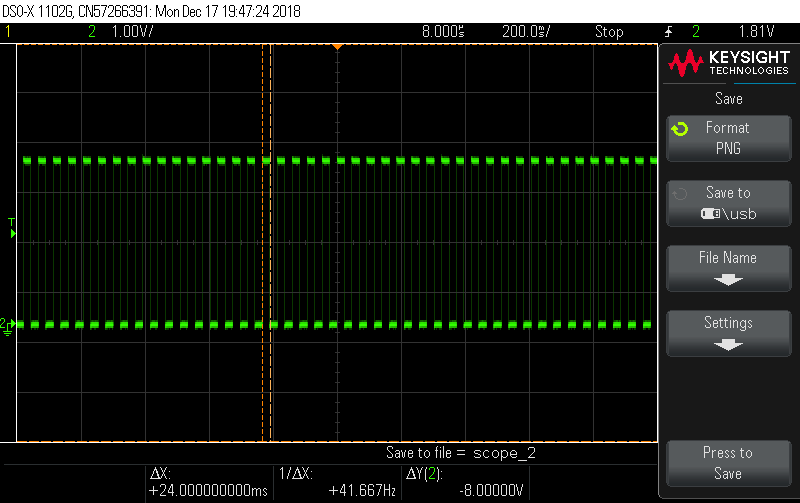
\includegraphics[width=1.2\textwidth]{figures/scope_2.png}}
    \caption{Capture of pin-toggles every time the sensor is sampled}
    \label{fig:sample_test}
\end{figure}

A small addition was added to the code, where it would invert a debug pin every time the sensor was sampled. This pin was then captured using a DSO, with the motors of the drones spinning at high speed to generate noise on the logic supply, and simulate flight. As can be seen, the sample-time was reliably 24 ms, with virtually no jitter in sample rate. This means our discretization of the sensor is still valid.

Another possible error we didn't test due to time constraints, was how the sensors distance readings performed at 400 mm distance, in flying conditions. We did consider saving these data, but the code already used the majority of the EEPROM to save the throttle data, and we didn't have any options to communicate with the drone-shim wirelessly.
Had time allowed it, a possible feature could've been added to the drone, keeping 1000 samples of height data in a ring buffer in RAM, as we still had plenty of RAM spare. 

\newpage

Final test

Simulations vs Test

Margin of error




























